\section{Nonnegative Variable Projection and Automatic Support Selection}\label{sec:algorithm}
\subsection{Conditional amplitudes and the exact local derivative}
For $r$ candidate rates, introduce dimensionless coordinates $z_j=\log(D_j/D_0)$ and a binary allowed-support matrix $H\in\{0,1\}^{r\times p}$. Conditional amplitudes solve
\begin{equation}\label{eq:nnls}
 A_H(z)\in\argmin_{A\geq0,\,A_{j\ell}=0\ \mathrm{if}\ H_{j\ell}=0}
 \tfrac12\|\sigma^{-1}(K(z)A-Y)\|_F^2,
 \quad \psi_H(z)=\tfrac12\|R_H(z)\|_F^2.
\end{equation}
Here $R_H=(KA_H-Y)/\sigma$. Rates are bounded by $[D_{\min},D_{\max}]$. Only selected signal frequencies enter this matrix problem; every retained frequency is fitted jointly. The method neither selects a single representative peak nor fits all 65,536 points of an otherwise sparse experimental spectrum indiscriminately.

With fixed rates and support, columns separate. If each allowed kernel submatrix has full column rank, the corresponding NNLS minimizer is unique. Without that condition, the fitted vector remains unique as the Euclidean projection onto a closed finitely generated cone, although the amplitudes can be nonunique. In exact arithmetic, enumerating all active subsets and selecting a feasible least-squares minimum solves the small NNLS problem. The implementation uses this strategy with SVD-based linear solves; it has exponential cost in $r$, so it is appropriate to the present cap of four rates, not to a dense 256-variable NNLS problem. The TRAIn-MF implementation instead calls MATLAB's \texttt{lsqnonneg}.

For allowed amplitudes, the Karush--Kuhn--Tucker conditions are
\begin{equation}\label{eq:kkt}
 A\geq0,\qquad G_A=K^\top(KA-Y)/\sigma^2\geq0,\qquad A\odot G_A=0.
\end{equation}
No sign condition on $G_A$ is required for coordinates fixed to zero by $H$: their feasible directions are absent. This distinction matters when auditing a screened solution.

\begin{Proposition}[Residual derivative on a stable active set]\label{prop:derivative}
Consider one column with locally unchanged positive active set $J$, full-column-rank $K_J$, and strict inactive inequalities. Set $a=K_J^+y$, $r=(K_Ja-y)/\sigma$, and $P_J=K_JK_J^+$. For an infinitesimal change $dK_J$,
\begin{equation}\label{eq:jacobian}
 dr=(I-P_J)(dK_J)a/\sigma-K_J^{+\top}(dK_J)^\top r.
\end{equation}
Consequently $d(\tfrac12\|r\|^2)=r^\top(dK_J)a/\sigma$.
\end{Proposition}
\begin{proof}
The active normal equations give $K_J^\top r=0$. Differentiating this identity and $\sigma r=K_Ja-y$ yields
$(K_J^\top K_J)da=-(dK_J)^\top\sigma r-K_J^\top(dK_J)a$.
Substitution into $dr$ gives Equation~\eqref{eq:jacobian}. Multiplication by $r^\top$, using $r^\top K_J=0$, gives the reduced differential.
\end{proof}

For a log-rate perturbation, $\partial K_{ij}/\partial z_j=-b_iD_j e^{-b_iD_j}$. The residual-dependent second term in Equation~\eqref{eq:jacobian} is retained. Dropping it changes the residual Jacobian even though the reduced objective gradient still has the envelope form. At active-set changes or rate collisions this smooth formula is not a differentiability theorem. A bounded trust-region reflective solver recomputes NNLS at every evaluation. In the archived code, $\log D_j$ is used directly; it differs from $z_j$ by a constant and has the same derivative.

Termination is checked through the library status, the amplitude KKT residual, and a scaled projected log-rate gradient. Specifically, with $g=J^\top\operatorname{vec}R$ and log-bound box $\mathcal B$, the recorded rate residual is
\begin{equation}\label{eq:stationarity}
 \eta_z=\frac{\|z-\Pi_{\mathcal B}(z-g)\|_\infty}
 {\max(1,\|J\|_2\|R\|_F)}.
\end{equation}
The denominator makes this a numerical diagnostic with an explicit scale, not a statistical precision guarantee. We require $\eta_z\leq10^{-6}$ and a relative amplitude KKT residual at most $10^{-7}$ for candidate eligibility. A failed candidate is recorded. These checks certify approximate first-order behavior of the attained candidate, not global minimization of the nonlinear problem or exhaustive support search.

\subsection{Spectral coherence through residualized kernels}\label{sec:screen}
Let the retained frequencies be partitioned into contiguous groups $G_1,\ldots,G_g$. For a candidate rate $D_j$, remove its column from $K$, writing the remaining matrix $K_{-j}$. Define
\begin{equation}\label{eq:score}
 v_j=(I-K_{-j}K_{-j}^+)k_j,\qquad
 Z_{jG}=\frac{\sum_{\ell\in G}v_j^\top y_\ell}
 {\sigma\|v_j\|_2\sqrt{|G|}}.
\end{equation}
The projection removes the linear span of the other candidate decays. It need not identify the true nuisance components. For fixed correct rates, it provides a useful elementary calculation.

\begin{Proposition}[Fixed-design screening identity]\label{prop:screen}
Suppose the rates and the frequency groups are fixed independently of iid Gaussian errors, the data follow $Y=KA+E$, and $v_j\ne0$. Then
\begin{equation}\label{eq:scoremean}
 Z_{jG}\sim N\left(
 \frac{\|v_j\|_2\sum_{\ell\in G}A_{j\ell}}{\sigma\sqrt{|G|}},1\right).
\end{equation}
If component $j$ is absent throughout $G$, its mean is zero. Testing $rg$ such fixed nulls at threshold $\Phi^{-1}(1-\alpha/(rg))$ controls the probability of at least one false rejection by $\alpha$.
\end{Proposition}
\begin{proof}
The nuisance term vanishes because $v_j^\top K_{-j}=0$, while $v_j^\top k_j=\|v_j\|_2^2$. Summing independent normal errors gives variance $|G|\sigma^2\|v_j\|_2^2$ before normalization. The final claim is the union bound and does not require independence between the different tests.
\end{proof}

When amplitudes are equal to $a$ in a group of $m$ frequencies, the mean score is $a\|v_j\|_2\sqrt m/\sigma$. Coherent small amplitudes can therefore be retained even if each is small relative to an unrelated tall peak. Adding frequencies with no component signal instead dilutes this score. As kernels become collinear, $\|v_j\|_2$ decreases, expressing the loss of separation information (Figure~\ref{fig:geometry}). With correlated spectral errors, the variance generally changes; replacing it by $m\sigma^2$ is not justified.

\begin{figure}[htbp]
\begin{adjustwidth}{-\extralength}{0cm}\centering
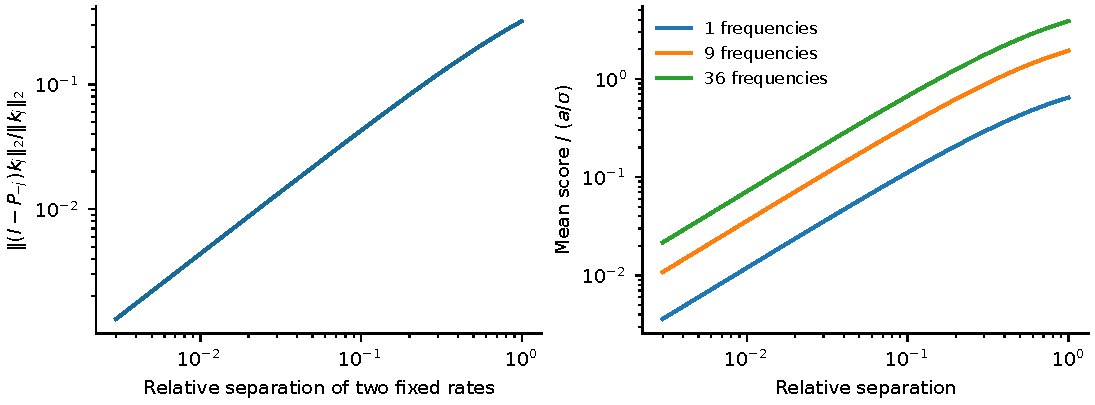
\includegraphics[width=\fulllength]{figures/geometry.pdf}
\caption{Fixed-design illustration of Equation~\eqref{eq:scoremean}, not a reconstruction benchmark. The two rates are $D/D_0=1$ and $1+\Delta$, with 32 equally spaced $bD_0$ values from 0 to 2.2. Left: the residualized-kernel norm decreases near collision. Right: coherent independent frequencies increase the expected standardized score by $\sqrt m$ for equal amplitudes. The rates and groups are fixed in this calculation.}\label{fig:geometry}
\end{adjustwidth}
\end{figure}

The operational screen estimates rates from the fitting data and groups frequencies after a signal mask. Consequently Proposition~\ref{prop:screen}'s calibration assumptions do not apply to the full estimator. We use $\alpha=0.01$ as a frozen screening parameter, not as a claimed family-wise error rate or chemical confidence level. If $\|v_j\|_2<10^{-10}\|k_j\|_2$, the implementation retains that component's allowed support: numerical nonidentifiability is not evidence of absence. Otherwise an entire group is allowed only when $Z_{jG}$ exceeds the threshold. NNLS still estimates separate nonnegative amplitudes at every retained frequency within an allowed group.

\subsection{Predictive comparison and automatic order}\label{sec:selection}
The available reconstruction rows are divided into an internal fitting set $T$ and an internal validation set $V$. Candidate paths include orders $0,1,\ldots,4$. For each path state, both the unrestricted support and, when different, the screened support are refined on $T$. A component with no allowed frequency is removed before refinement. Let $\widehat Y_{c,V}$ denote a candidate's prediction on $V$, and put
\begin{equation}\label{eq:val}
 L_c=\|\widehat Y_{c,V}-Y_V\|_F^2/\sigma^2.
\end{equation}
For numerically eligible candidates, let $c_*$ minimize $L_c$. We retain the set
\begin{equation}\label{eq:selection}
 \mathcal E=\left\{c:L_c\leq L_{c_*}+
 2\|\widehat Y_{c,V}-\widehat Y_{c_*,V}\|_F/\sigma+10^{-10}\right\}.
\end{equation}
Within $\mathcal E$, selection is lexicographic: fewer surviving rates, then fewer allowed amplitudes, then lower validation loss. The selected fixed support is refitted on $T\cup V$. The zero-signal model is a legitimate candidate. The selected $r$ is therefore automatic within a declared finite search, without access to the true order. Attaining the cap is reported rather than interpreted as evidence that no additional rates exist.

\begin{Proposition}[Conditional paired prediction variance]\label{prop:paired}
Let $P,Q$ be fixed predictions independent of $E$, and $Y=M+E$ with iid $N(0,\sigma^2)$ errors. Then
\begin{align}
 \mathbb E\{(\|P-Y\|_F^2-\|Q-Y\|_F^2)/\sigma^2\}
 &= (\|P-M\|_F^2-\|Q-M\|_F^2)/\sigma^2,\label{eq:pairedbias}\\
 \operatorname{Var}\{(\|P-Y\|_F^2-\|Q-Y\|_F^2)/\sigma^2\}
 &=4\|P-Q\|_F^2/\sigma^2.\label{eq:pairedvar}
\end{align}
\end{Proposition}
\begin{proof}
Subtracting the losses cancels the quadratic error term. The random remainder is $-2\langle P-Q,E\rangle/\sigma^2$, a centered normal variable with the variance in Equation~\eqref{eq:pairedvar}.
\end{proof}

This identity motivates the one-standard-deviation allowance in Equation~\eqref{eq:selection}; it does not provide a simultaneous confidence set after choosing the best of many candidates. Moreover, the benchmark signal mask uses all outer training rows, some of which become internal validation rows. Conditional independence of predictions and internal validation noise is therefore not exact after masking. The internal rule is explicitly heuristic. The eight external test acquisitions remain unused in the mask, candidate fitting, and selection, preserving an independent predictive evaluation for this full procedure. A future inferential version would need independent masking or cross-fitting and selection-adjusted calibration; neither has been retroactively attributed to the frozen benchmark.

\begin{Algorithm}[Spectral-support selection]
Given observed $b,Y,\sigma$, retained frequencies and physical bounds:
\begin{enumerate}
\item Sort the distinct acquisition coordinates and reserve internal validation rows. Construct groups from frequency coordinates without crossing large gaps.
\item Generate the native RAI or DOME path on internal fitting rows for orders zero to four.
\item For each state, construct the unrestricted and screened supports. Refine each through NNLS variable projection on fitting rows; save failures and diagnostics.
\item Predict internal validation rows, select by Equation~\eqref{eq:selection}, and apply the stated complexity tie-break.
\item Refit on all supplied outer training rows. Return rates, amplitudes, support, candidate losses, numerical diagnostics, and the automatically selected order. Export a mass-conserving 256-bin map for display.
\end{enumerate}
\end{Algorithm}

\subsection{The roles of RAI, DOME, TRAIn-MF, and TRAIn}
RAI's component path uses deterministic multistart nonnegative variable projection, including residual-based births, and its original selector minimizes a known-noise BIC-type score
$\mathrm{RSS}/\sigma^2+r(p+1)\log(np)$. All amplitudes are counted, including zeros. This is a heuristic adaptation of regular-model information criteria \cite{schwarz}: zero amplitudes and coincident rates create singular parameterizations. Singular learning theory explains why regular-model parameter-count penalties need not retain their usual interpretation in such settings \cite{watanabe}; we use these scores as documented heuristics.

DOME uses variance-based split proposals, frequency-dependent residual contrasts, and pairwise moment exchanges, followed by exact-kernel refinement. For example, splitting a mass $A$ at $m$ into $pA$ at $m-(1-p)\Delta$ and $(1-p)A$ at $m+p\Delta$ preserves mass and first moment, with
\begin{equation}\label{eq:split}
 Y_{\mathrm{split}}(b)-Ae^{-bm}
 =\tfrac12 Ae^{-bm}b^2p(1-p)\Delta^2+O(\Delta^3).
\end{equation}
This gives a proposal direction; every candidate is judged using the exact exponential model. The native DOME score is $\mathrm{RSS}/\sigma^2+2d+2d(d+1)/\max(np-d-1,1)$, where $d$ counts numerically positive amplitudes plus rates. It is also heuristic. RAI-S and DOME-S replace these native final order decisions with the same support/prediction procedure, while retaining their different candidate paths. Agreement between their outputs is not two independent demonstrations of benefit. No ablation here establishes a specific advantage of DOME's moment mechanism.

The archived TRAIn-MF solves a different problem. The suffix MF in TRAIn-MF is used in the multifrequency sense of the historical \texttt{TRAIn\_DOSY\_MFV31} header. Its matrix factorization $Y\approx KSA$ shares diffusion profiles (columns of $S$) across chemical shifts while allowing different component spectra (rows of $A$). It remains multifrequency when $r=1$: multiple frequencies need not imply multiple components. This terminology preserves the source lineage without equating the later constrained solver with the original TRAIn iteration. With $\widetilde Y=Y/s_Y$, $s_Y=\|Y\|_F/\sqrt{np}$ for nonzero data, its objective is
\begin{equation}\label{eq:mf}
 F(S,A)=\frac{\|KSA-\widetilde Y\|_F^2}{2p}
 +\frac{\lambda_S}{2}\|LS\|_F^2
 +\frac{\lambda_A}{2p}\|A\|_F^2,
\end{equation}
subject to Equation~\eqref{eq:mfconstraints}. Here $L$ discretizes density curvature on the log-diffusion grid, including mass-to-density conversion and quadrature weights. The reference uses 256 masses and $\lambda_S=\lambda_A=10^{-8}$. Conditional $A$ updates are augmented MATLAB NNLS problems; conditional $S$ updates enforce simplex constraints, and reduced-profile refinement follows if stationarity is inadequate. Monotone accepted objective values, being bounded below, converge as scalar values. This observation alone does not establish convergence of the factors or global optimality; KKT checks remain necessary. Block-coordinate convergence results require additional hypotheses on the objective and subproblem solutions \cite{tseng}. We do not assert that citing such a result establishes those hypotheses for every step of the archived solver.

The automatic TRAIn-MF selector first counts noise-resolved singular directions, caps the factor search at four and at that count, and then uses paired held-out losses among numerically converged candidates. Its count describes resolved predictive factors, with the limitation in Proposition~\ref{prop:rank}. The TRAIn-MF is included here as an unchanged distributional reference on a previously saved example, not as a newly tested winner on the atomic test. The provenance of this TRAIn-MF research line is explicit: the original TRAIn of Xu and Zhang \cite{train} was extended to a shared multifrequency model by Arrabal-Campos in \texttt{TRAIn\_DOSY\_MFV31} \cite{mfv31}. The archived source identifies its author and embeds a TRAIn-derived component solver using $h=\eta^2$, a Gauss--Newton model, truncated conjugate gradients, and trust-radius updates based on actual versus predicted reduction. This is a direct algorithmic antecedent of the TRAIn-MF extension, not an attribution inferred merely from a generic trust-region call.

The later TRAIn-MF reference used here replaces that embedded iteration with the constrained updates and stationarity checks associated with Equation~\eqref{eq:mf}. Thus the benchmarked solver and historical Version 3.1 differ numerically, while the TRAIn-MF lineage and authorship remain acknowledged. The public repository preserves both files and their identities \cite{software}. RAI-S and DOME-S use separate proposal mechanisms and a common support selector; a generic trust-region step does not by itself make either method an implementation of the original TRAIn.
